\chapter{Differentiation and Edge Detection}
\label{ch:lesson12}

An edge is, informally, a place where intensity changes quickly. That's a statement about a \emph{derivative}. This chapter builds up discrete image derivatives --- Prewitt, Sobel, and Scharr operators --- as convolution kernels (Chapter~\ref{ch:lesson10}), uses them inside the classic \textbf{Canny} edge detector, and finishes by turning the resulting edge maps into actual shapes with the \textbf{Hough transform}.

\section{From derivatives to gradients}

Treat the image as a function $I(x,y)$. Its gradient $\nabla I=(I_x,I_y)$ points in the direction of steepest intensity increase, where $I_x=\partial I/\partial x$ and $I_y=\partial I/\partial y$ are the \textbf{partial derivatives} of image intensity --- how fast the intensity changes as you move one pixel right, or one pixel down. Two numbers summarize the gradient at each pixel:
\begin{itemize}
  \item \textbf{magnitude} $\|\nabla I\| = \sqrt{I_x^2+I_y^2}$ --- how sharp the change is (large at edges, near zero on flat regions)
  \item \textbf{direction} $\theta = \operatorname{atan2}(I_y,I_x)$ --- which way intensity is increasing fastest (perpendicular to the edge)
\end{itemize}
$I_x$ and $I_y$ are themselves computed by convolving the image with small derivative kernels.

\section{Prewitt, Sobel, and Scharr: derivative + smoothing}

The simplest $I_x$ estimate is a 1D central-difference kernel $[-1,\,0,\,1]$; it works, but with no smoothing in the perpendicular direction, it's maximally sensitive to noise. Real operators combine a difference in one direction with a \emph{smoothing} average in the perpendicular direction --- this is what makes them robust to noise. They differ only in how they weight that smoothing:

\begin{center}
\begin{tabular}{lll}
\hline
\textbf{Operator} & $x$\textbf{-kernel} & \textbf{Perpendicular weighting} \\
\hline
Prewitt & $\begin{bmatrix}-1&0&1\\-1&0&1\\-1&0&1\end{bmatrix}$ & uniform: 1, 1, 1 \\[1.2em]
Sobel & $\begin{bmatrix}-1&0&1\\-2&0&2\\-1&0&1\end{bmatrix}$ & binomial: 1, 2, 1 \\[1.2em]
Scharr & $\begin{bmatrix}-3&0&3\\-10&0&10\\-3&0&3\end{bmatrix}$ & 3, 10, 3 \\
\hline
\end{tabular}
\end{center}

Each $y$-kernel is just the transpose of its $x$-kernel. Sobel's binomial weights approximate a small Gaussian, which is why it's the most commonly used default. Scharr's weights were numerically optimized specifically to make the \emph{estimated gradient direction} as rotationally accurate as possible --- which matters most in applications like optical flow that depend on precise gradient angles rather than just edge location. Figure~\ref{fig:l12-1} compares all four operators.

\begin{figure}[h]
\centering
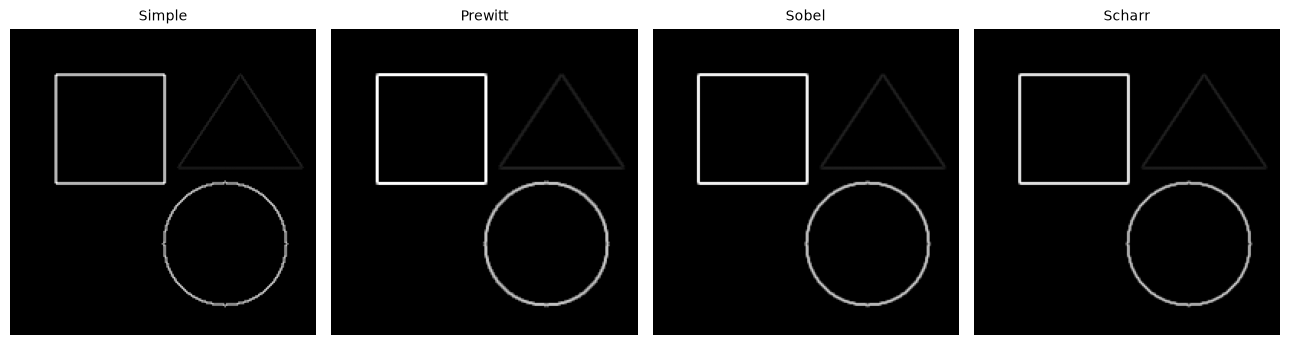
\includegraphics[width=0.95\textwidth]{figures/lesson12_fig03.png}
\caption{Gradient magnitude from the simple difference kernel and the three smoothed operators, on a clean test image. On a low-noise image like this, the four results look nearly identical.}
\label{fig:l12-1}
\end{figure}

\subsection*{Noise robustness: why the perpendicular smoothing matters}

To make the benefit of perpendicular smoothing concrete, measure each kernel's response to pure noise on a flat (edge-free) region, after first rescaling each kernel to the \emph{same gain} on an ideal step edge (dividing by the sum of its positive weights) so a kernel with larger raw coefficients doesn't look noisier just from its overall scale.

\begin{center}
\renewcommand{\arraystretch}{1.4}
\begin{tabular}{lr}
\hline
\textbf{Kernel} & \textbf{Noise std (gain-normalized)} \\
\hline
Simple $[-1,0,1]$ & 20.93 \\
Prewitt & 12.29 \\
Sobel & 12.97 \\
Scharr & 14.32 \\
\hline
\end{tabular}
\end{center}

The plain difference kernel is noticeably noisier than any of the $3\times3$ operators --- averaging over 3 rows (or columns) while differencing cuts down the noise response substantially, which is exactly the point of building smoothing into the derivative kernel.

\section{From gradients to edges: the Canny detector}

Simply thresholding gradient magnitude gives thick, noisy edge blobs. The \textbf{Canny} edge detector (\citelink{canny1986}{Canny, 1986}) refines this with a multi-stage pipeline:
\begin{enumerate}
  \item \textbf{Smooth} with a Gaussian, to suppress noise before differentiating.
  \item \textbf{Compute gradients} (Sobel, internally) to get magnitude and direction at every pixel.
  \item \textbf{Non-maximum suppression}: at each pixel, keep the gradient magnitude only if it's a local maximum \emph{along the gradient direction} --- this thins wide gradient ridges down to single-pixel-wide lines.
  \item \textbf{Double thresholding + hysteresis}: pixels above a high threshold are definite edges; pixels below a low threshold are discarded; pixels in between are kept only if they connect to a definite edge.
\end{enumerate}
Figure~\ref{fig:l12-2} compares the naive and Canny results.

\begin{figure}[h]
\centering
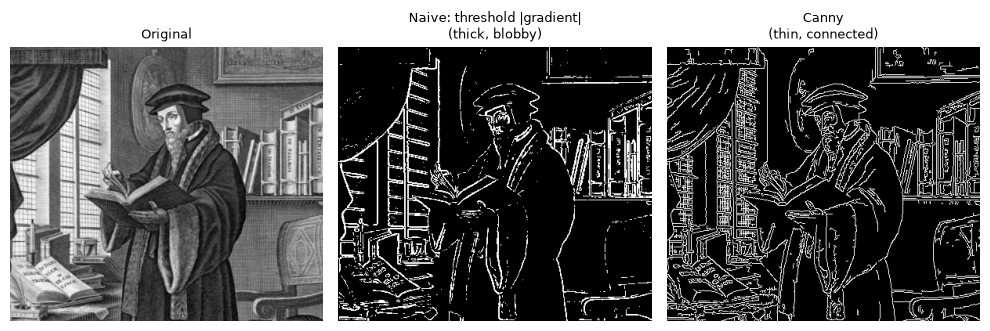
\includegraphics[width=0.9\textwidth]{figures/lesson12_fig04.png}
\caption{Naively thresholding $\|\nabla I\|$ gives thick, blobby edges; \code{cv2.Canny} gives thin, connected ones. \attrib{Image source: \href{https://www.nga.gov/artworks/37890-john-calvin}{National Gallery of Art}.}}
\label{fig:l12-2}
\end{figure}

\subsection*{Threshold sensitivity}

Canny's two thresholds trade off completeness against noise. Too low, and noise gets picked up as spurious edges; too high, and real (but low-contrast) edges are missed, as Figure~\ref{fig:l12-3} shows.

\begin{figure}[h]
\centering
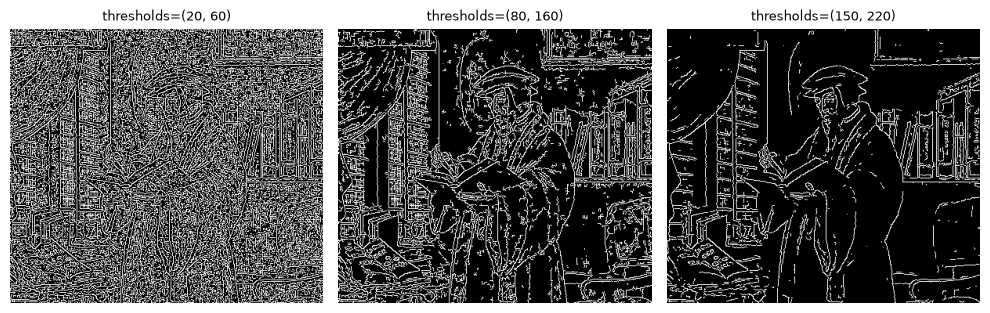
\includegraphics[width=0.9\textwidth]{figures/lesson12_fig05.png}
\caption{With low thresholds on a noisy image, speckle noise survives as spurious edge fragments. At the highest thresholds, faint detail disappears completely, while the strongest outlines survive --- Canny's threshold trading off noise rejection against sensitivity to faint-but-genuine edges.}
\label{fig:l12-3}
\end{figure}

\section{From edges to lines: the Hough transform}

Edge detection finds \emph{where} intensity changes sharply, but it doesn't know that a scattered set of edge pixels forms a straight line. The \textbf{Hough transform} (\citelink{hough1962}{Hough, 1962}; \citelink{dudahart1972}{Duda \& Hart, 1972}) answers a different question: given a set of edge points, which ones are consistent with lying on a common line?

Parameterize a line not as $y=mx+b$ (which blows up for vertical lines) but by its distance from the origin and the angle of its normal:
\begin{equation}
\rho = x\cos\theta + y\sin\theta.
\end{equation}
For a \emph{fixed} edge point $(x,y)$, this traces a sinusoidal curve in $(\rho,\theta)$ space as $\theta$ varies --- every $(\rho,\theta)$ pair on that curve describes a line through $(x,y)$. The key idea: if several edge points are \textbf{collinear}, their sinusoids all cross at the \emph{same} $(\rho,\theta)$ --- the parameters of the line they share, as demonstrated in Figure~\ref{fig:l12-4}.

\begin{figure}[h]
\centering
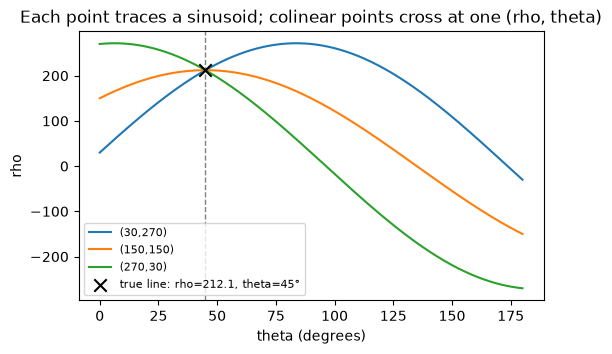
\includegraphics[width=0.55\textwidth]{figures/lesson12_fig06.png}
\caption{Three points on the line $x+y=300$ each trace a sinusoid in $(\rho,\theta)$ space; all three cross at the line's true parameters, $\rho=212.1$, $\theta=45^\circ$.}
\label{fig:l12-4}
\end{figure}

\subsection*{The accumulator: voting for lines}

In practice, every edge pixel votes for its entire sinusoid of possible $(\rho,\theta)$ lines, into a discretized 2D \textbf{accumulator} array; the bin with the most votes is the line most consistent with the data. Built from scratch for a single synthetic line and checked against \code{cv2.HoughLines}: the manual accumulator peak lands at $\rho=212$, $\theta=45.0^\circ$, and \code{cv2.HoughLines} reports $\rho=211$, $\theta=45.0^\circ$ --- both within a pixel of the true $\rho=212.1$. Figure~\ref{fig:l12-5} shows the accumulator and recovered line.

\begin{figure}[h]
\centering
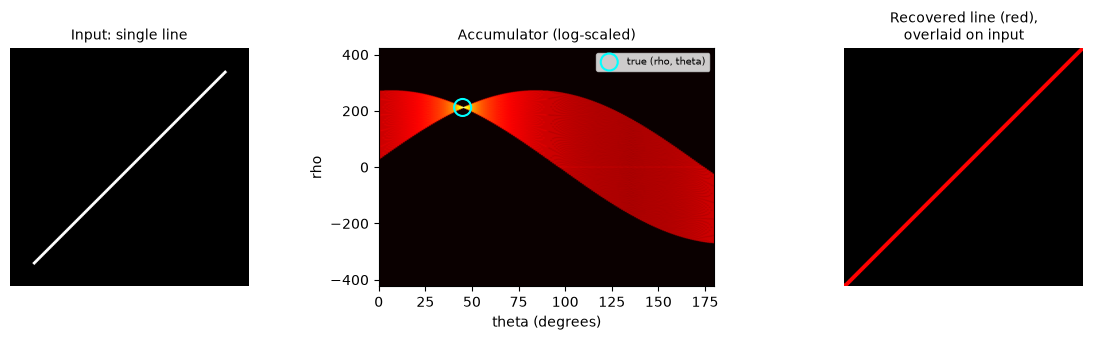
\includegraphics[width=0.95\textwidth]{figures/lesson12_fig07.png}
\caption{Input line, the log-scaled $(\rho,\theta)$ accumulator (true parameters marked in cyan), and the recovered line overlaid in red. The basic Hough transform returns an infinite line, not a line segment.}
\label{fig:l12-5}
\end{figure}

\subsection*{\code{cv2.HoughLinesP}: the practical version}

The probabilistic Hough transform additionally returns line \emph{segment} endpoints, and is what's normally used in practice, run on top of an actual Canny edge map, as in Figure~\ref{fig:l12-6}.

\begin{figure}[h]
\centering
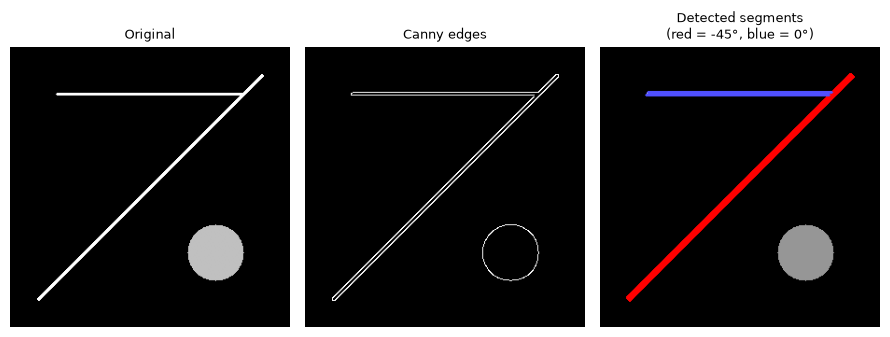
\includegraphics[width=0.85\textwidth]{figures/lesson12_fig08.png}
\caption{Two lines (true angles $-45^\circ$ and $0^\circ$) plus a distractor circle with no straight edges. Every detected segment lands almost exactly on one of the two true angles; the circle correctly produces no line detections. Each line typically yields two or three near-duplicate detections, since Canny finds an edge on \emph{each} side of a stroke with finite width.}
\label{fig:l12-6}
\end{figure}

\subsection*{Beyond lines: Hough circles}

The same voting idea generalizes to any shape describable by a small number of parameters. A circle needs 3 (center $x$, center $y$, radius $r$), so \code{cv2.HoughCircles} accumulates votes in a 3D parameter space instead of 2D. For a true circle at center $(100,100)$, radius $50$: \code{cv2.HoughCircles} reports center $(98.5, 100.5)$, radius $50.0$, shown in Figure~\ref{fig:l12-7}.

\begin{figure}[h]
\centering
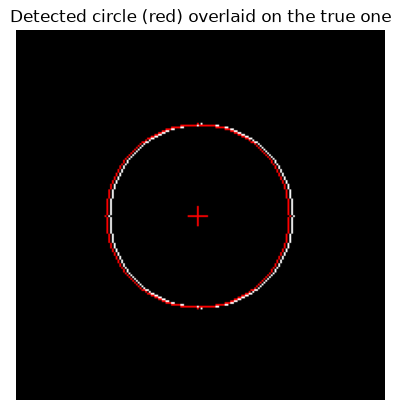
\includegraphics[width=0.35\textwidth]{figures/lesson12_fig09.png}
\caption{Detected circle (red) overlaid on the true one (white).}
\label{fig:l12-7}
\end{figure}

\code{cv2.HoughCircles} doesn't expose its internal accumulator, but building one from scratch follows the same voting idea, with one more dimension: each edge pixel votes for every $(c_x,c_y,r)$ triple it could be consistent with, for every candidate radius. A from-scratch accumulator peak lands at center $(100,100)$, radius $51$ --- matching the true circle almost exactly, visualized in Figure~\ref{fig:l12-8}.

\begin{figure}[h]
\centering
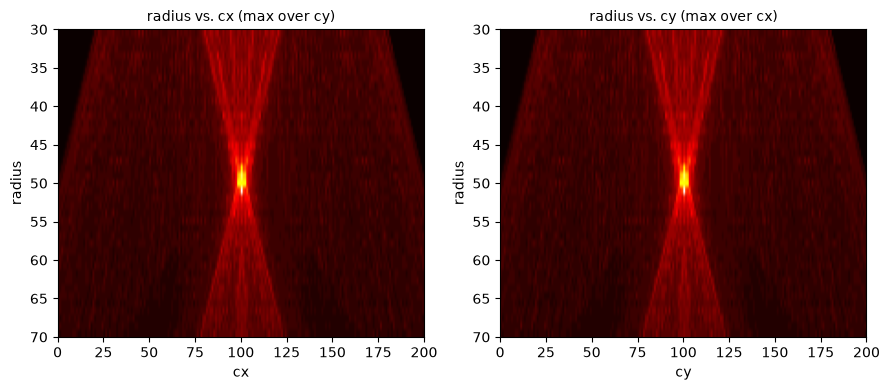
\includegraphics[width=0.85\textwidth]{figures/lesson12_fig10.png}
\caption{2D slices of the 3D circle accumulator: radius vs.\ $c_x$ (max over $c_y$) and radius vs.\ $c_y$ (max over $c_x$). Each slice shows a bright X where every edge point's votes cross at the true center and radius.}
\label{fig:l12-8}
\end{figure}

\subsection*{Exercises}
\begin{enumerate}
  \item Increase the noise standard deviation in \code{flat\_noisy} and re-run the noise-robustness comparison. Does the relative ordering of the four kernels change?
  \item \code{cv2.Canny} accepts an \code{apertureSize} parameter for its internal Sobel step (default 3). Try \code{apertureSize=5} and compare the result to the default on the noisy image.
  \item Canny's hysteresis step needs a \emph{connected} path of above-low-threshold pixels between a weak edge and a strong one. Construct a small binary example (by hand, as a NumPy array) where a real edge is broken into two segments with a 1-pixel gap, and confirm that hysteresis fails to link them even though a human viewer would clearly see one edge.
  \item Lower \code{cv2.HoughLinesP}'s \code{threshold} argument well below 60 on the two-line scene. Do you start getting spurious short segments from noise in the circle's Canny boundary, even though it has no straight edges? What does raising \code{minLineLength} do to fix this?
  \item Add a third line at a shallow angle (e.g.\ from $(30,200)$ to $(270,150)$), and predict its angle before checking \code{HoughLinesP}'s output against your prediction.
  \item \code{cv2.HoughCircles}'s \code{param2} argument is roughly an accumulator vote threshold --- lower values report more (and more spurious) circles. Sweep \code{param2} from 30 down to 10 on a noisy version of the circle image and observe when false-positive circles start appearing.
\end{enumerate}

\vfill
\fullcode{lesson12}{lesson12_differentiation_edges}
